%!TEX TS-program = xelatex
 
% Этот шаблон документа разработан в 2014 году
% Данилом Фёдоровых (danil@fedorovykh.ru) 
% для использования в курсе 
% <<Документы и презентации в \LaTeX>>, записанном НИУ ВШЭ
% для Coursera.org: http://coursera.org/course/latex .
% Исходная версия шаблона --- 
% https://www.writelatex.com/coursera/latex/5.2.2
 
\documentclass[a4paper,12pt]{article}
 
%%% Работа с русским языком
\usepackage[english]{babel}   %% загружает пакет многоязыковой вёрстки
\usepackage{fontspec}      %% подготавливает загрузку шрифтов Open Type, True Type и др.
\defaultfontfeatures{Ligatures={TeX},Renderer=Basic}  %% свойства шрифтов по умолчанию
\setmainfont[Ligatures={TeX,Historic}]{Times New Roman} %% задаёт основной шрифт документа
\setsansfont{Comic Sans MS}                    %% задаёт шрифт без засечек
\setmonofont{Courier New}
\usepackage{indentfirst}
\frenchspacing
 
\renewcommand{\epsilon}{\ensuremath{\varepsilon}}
\renewcommand{\phi}{\ensuremath{\varphi}}
\renewcommand{\kappa}{\ensuremath{\varkappa}}
\renewcommand{\le}{\ensuremath{\leqslant}}
\renewcommand{\leq}{\ensuremath{\leqslant}}
\renewcommand{\ge}{\ensuremath{\geqslant}}
\renewcommand{\geq}{\ensuremath{\geqslant}}
\renewcommand{\emptyset}{\varnothing}
 
%%% Дополнительная работа с математикой
\usepackage{amsmath,amsfonts,amssymb,amsthm,mathtools} % AMS
\usepackage{icomma} % "Умная" запятая: $0,2$ --- число, $0, 2$ --- перечисление
 
%% Номера формул
%\mathtoolsset{showonlyrefs=true} % Показывать номера только у тех формул, на которые есть \eqref{} в тексте.
%\usepackage{leqno} % Нумерация формул слева
 
%% Свои команды
\DeclareMathOperator{\sgn}{\mathop{sgn}}
 
%% Перенос знаков в формулах (по Львовскому)
\newcommand*{\hm}[1]{#1\nobreak\discretionary{}
{\hbox{$\mathsurround=0pt #1$}}{}}
 
%%% Работа с картинками
\usepackage{graphicx}  % Для вставки рисунков
\graphicspath{{images/}{images2/}}  % папки с картинками
\setlength\fboxsep{3pt} % Отступ рамки \fbox{} от рисунка
\setlength\fboxrule{1pt} % Толщина линий рамки \fbox{}
\usepackage{wrapfig} % Обтекание рисунков текстом
 
%%% Работа с таблицами
\usepackage{array,tabularx,tabulary,booktabs} % Дополнительная работа с таблицами
\usepackage{longtable}  % Длинные таблицы
\usepackage{multirow} % Слияние строк в таблице
 
%%% Теоремы
\theoremstyle{plain} % Это стиль по умолчанию, его можно не переопределять.
\newtheorem{theorem}{Теорема}[section]
\newtheorem{proposition}[theorem]{Утверждение}
 
\theoremstyle{definition} % "Определение"
\newtheorem{corollary}{Следствие}[theorem]
\newtheorem{problem}{Задача}[section]
 
\theoremstyle{remark} % "Примечание"
\newtheorem*{nonum}{Решение}
 
%%% Программирование
\usepackage{etoolbox} % логические операторы
 
 
%%% Страница
\usepackage{extsizes} % Возможность сделать 14-й шрифт
\usepackage{geometry} % Простой способ задавать поля
	\geometry{top=5mm}
	\geometry{bottom=15mm}
	\geometry{left=5mm}
	\geometry{right=5mm}
 %
%\usepackage{fancyhdr} % Колонтитулы
% 	\pagestyle{fancy}
 	%\renewcommand{\headrulewidth}{0pt}  % Толщина линейки, отчеркивающей верхний колонтитул
% 	\lfoot{Нижний левый}
% 	\rfoot{Нижний правый}
% 	\rhead{Верхний правый}
% 	\chead{Верхний в центре}
% 	\lhead{Верхний левый}
%	\cfoot{Нижний в центре} % По умолчанию здесь номер страницы
 
\usepackage{setspace} % Интерлиньяж
%\onehalfspacing % Интерлиньяж 1.5
%\doublespacing % Интерлиньяж 2
%\singlespacing % Интерлиньяж 1
 
\usepackage{lastpage} % Узнать, сколько всего страниц в документе.
 
\usepackage{soul} % Модификаторы начертания
 
\usepackage{hyperref}
\usepackage[usenames,dvipsnames,svgnames,table,rgb]{xcolor}
\hypersetup{				% Гиперссылки
    unicode=true,           % русские буквы в раздела PDF
    pdftitle={Заголовок},   % Заголовок
    pdfauthor={Автор},      % Автор
    pdfsubject={Тема},      % Тема
    pdfcreator={Создатель}, % Создатель
    pdfproducer={Производитель}, % Производитель
    pdfkeywords={keyword1} {key2} {key3}, % Ключевые слова
    colorlinks=true,       	% false: ссылки в рамках; true: цветные ссылки
    linkcolor=red,          % внутренние ссылки
    citecolor=black,        % на библиографию
    filecolor=magenta,      % на файлы
    urlcolor=cyan           % на URL
}
 
\usepackage{csquotes} % Еще инструменты для ссылок
 
%\usepackage[style=authoryear,maxcitenames=2,backend=biber,sorting=nty]{biblatex}
 
\usepackage{multicol} % Несколько колонок
 
\usepackage{tikz} % Работа с графикой
\usepackage{pgfplots}
\usepackage{pgfplotstable}
 
\author{Batarin Egor, Beksultanova Aikun, Zubritsky Ivan}
\title{Feed-forward neuronet recognising digits}
\date{\today}
 
\begin{document} % конец преамбулы, начало документа
 
\maketitle
 
\begin{abstract}
   This pdf is done to descript the neuronet architecture and give step-by-step description of learning algorithms.
\end{abstract}
\section{Accepted notations}

$x \in \mathbb {R}^p$ - input value of neuronet, $p = \text{lenght} \times \text{width}$ - number of image pixels. $x$ consists of $0$ - "white color" and $1$ - "black color".

$y = y(x) \in \mathbb {R}^{10}$ - desired output value. If input $x$ responds to a digit $i \in \{0, 1, ... , 9\}$, then $y(x)$ consists of nine zeros, and one, which is in a $i$-th place.

$L$ - number of the last (output) layer.

$n:\left\{ {1, \ldots ,L} \right\} \to \mathbb {N}$ - number of neurons in the $l$-th layer, $n(1) = p$, $n(L) = 10$.


\[{\omega ^l} = \left( \begin{array}{l}
\begin{array}{*{20}{c}}
{w_{11}^l} & {w_{12}^l} & ... & {w_{1,n(l-1)}^l} \\
{w_{21}^l} & {w_{22}^l} & ... & {w_{2,n(l-1)}^l} \\
...     &     ...    & ... & ... \\
{w_{j1}^l} & {w_{j2}^l} & ... & {w_{j,n(l-1)}^l}\\
...     &     ...    & ... & ... \\
{w_{n(l),1}^l} & {w_{n(l),2}^l} & ... & {w_{n(l),n(l-1)}^l} 
\end{array}\\

\end{array} \right)\]
$w^l$ is weight matrix, which consist of $w_{jk}^l$ - weight between $j$-th neuron in $l$ layer and $k$-th
neuron in $l-1$ layer. $l = 2, \ldots, L$.


${b^l} = {\left( {b_1^l,b_2^l, \ldots, b_{n(l)}^l} \right)^T}$ is a vector of biases, ${b_j^l}$ - bias of $j$-th neuron in the $l$-th layer. $l = 2, \ldots, L$.

${a^l} = {\left( {a_1^l,a_2^l, \ldots, a_{n(l)}^l } \right)^T}$ is a vector of activations, ${b_j^l}$ - bias of $j$-th neuron in the $l$-th layer, $x = a^1 \in \mathbb {R}^p$ - input value, $a^L \in \mathbb  {R}^{10}$ - output value, predicted by neuronet. $l = 1, \ldots, L$.

We define weighted input vector ${z^l} = \left( {z_1^l,z_2^l, \ldots ,z_{n(l)}^l} \right)$, where $z_j^l = \sum\limits_{k = 1}^{n(l - 1)} {\omega _{jk}^la_k^{l - 1} + b_j^l}$. It can be written in vectorized form $z^l = \omega^la^{l-1}+b^l$. $l = 2, \ldots, L$.

${C_{\text{quad}}}(x) = \frac{1}{2}\left\| {y(x) - {a^L}(x)} \right\| = \frac{1}{2}\sqrt {\sum\limits_{i = 1}^{10} {{{\left( {{y_i}(x) - a_i^L(x)} \right)}^2}} } $ is quadratic cost, refered to a single input value $x$.

We will also use cross-entropy cost $C_\text{log}(x) =  - \sum\limits_{i = 1}^{10} {{y_i}(x)\ln a_i^L(x) + \left( {1 - {y_i}(x)} \right)\ln } \left( {1 - a_i^L(x)} \right)$

$\sigma (z) = \frac{1}{{1 + {e^{ - z}}}}$ - sigmoid activation function, $\sigma '(z) = \sigma (z)\left( {1 - \sigma (z)} \right)$. This funtion links activation and weighted input: $a^l = \sigma(z^l)$, $l = 2, \ldots, L$.

For any cost function we define ${\nabla _a}C = {\left( {\frac{{\partial C}}{{\partial z_1^L}}, \cdots ,\frac{{\partial C}}{{\partial z_{10}^L}}} \right)^T}$, $C = \frac{1}{{\text{number of inputs}}}\sum\limits_x {C(x)}$ - average cost.

For two vectors $a = {\left( {{a_1},{a_2}, \ldots ,{a_n}} \right)^T}$ and $b = {\left( {{b_1},{b_2}, \ldots ,{b_n}} \right)^T}$ the Hadamard product $a \odot b$ is defined as \[a \odot b=  {\left( {{a_1b_1},{a_2b_2}, \ldots ,{a_nb_n}} \right)^T} \]

We define an error $\delta _j^l$ of $j$-th neuron in $l$-th layes as $\delta _j^l = \frac{{\partial C}}{{\partial z_j^l}}$, $\delta^l = {\left( \delta _1^l, \ldots, \delta _{n(l)}^l \right)^T}$. $l = 2, \ldots, L$.

\newpage
\section{Neuronet architecture}

The structure of neuronet is presented in the picture below:

\begin{figure}[h!]
	\begin{center}
		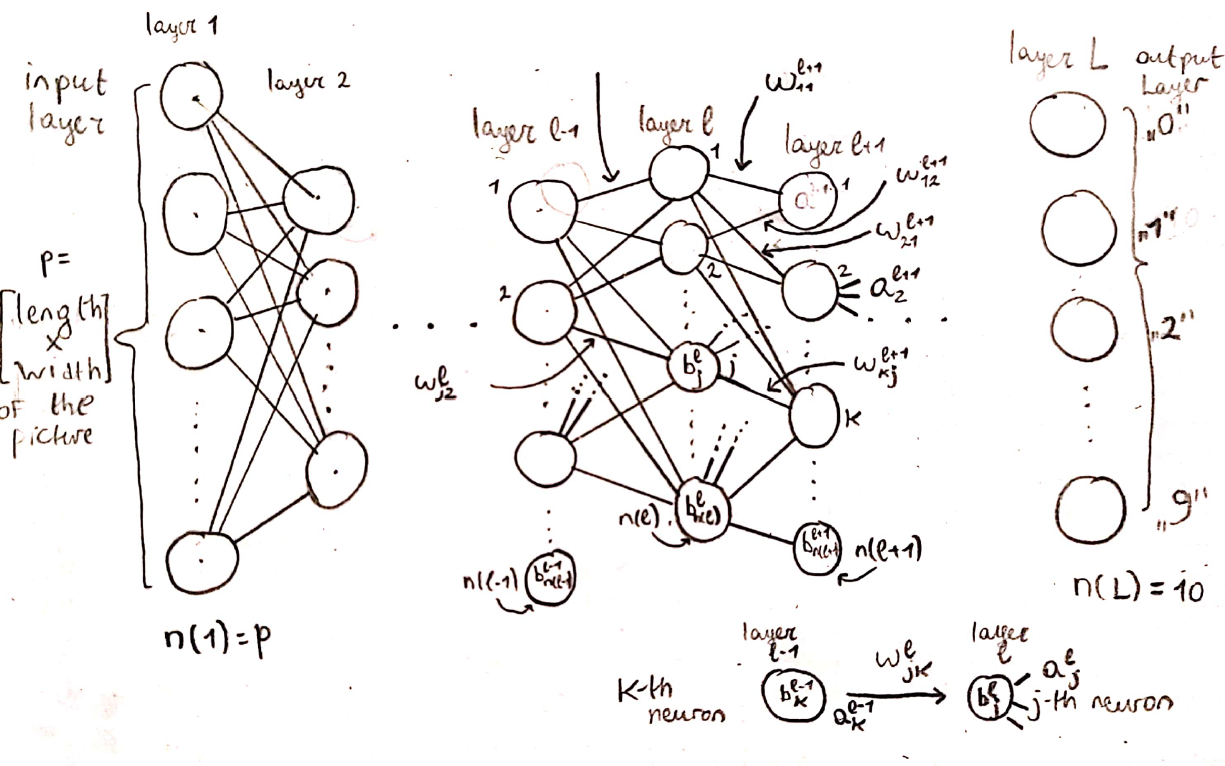
\includegraphics[scale = 0.75]{1.png}
		\caption{Neuronet structure}
		\label{p1}
	\end{center}
\end{figure}
\section{Backpropagation equations}

Below four significant equations are presented, which will be used in backpropagation algorithm:

\begin{equation}\label{eq:1}
{\delta ^L} = {\nabla _a}C \odot \sigma '({z^L})
\end{equation}


\begin{equation}\label{eq:2}
{\delta ^l} = \left( {{{\left( {{\omega ^{l + 1}}} \right)}^T}{\delta ^{l + 1}}} \right) \odot \sigma '({z^l})
\end{equation}


\begin{equation}\label{eq:3}
\frac{{\partial C}}{{\partial b_j^l}} = \delta _j^l
\end{equation}


\begin{equation}\label{eq:4}
\frac{{\partial C}}{{\partial \omega _{jk}^l}} = a_k^{l - 1}\delta _j^l
\end{equation}
\newpage
\section{Learning algorithm}
\begin{enumerate}
	\item \textbf{Set hyper-parameters}: learning rate $\eta$, number $N$ of epoch of training, size $m$ of mini-batch.
	\item \textbf{Repeat for each of $N$-th epochs of training}:
	\begin{enumerate}
		\item \textbf{Input a random mini-batch of $m$ training examples $x$ from training data}.
		\item \textbf{For each training example} $x$: Set the corresponding input activation $a^{x,1} = x$, a do the following:
		\begin{enumerate}
			\item \textbf{Feedforward}: For each $l = 2, 3, \ldots, L$ compute $z^{x,l} = \omega^la^{x,l-1}+b^l$ and $a^{x,l} = \sigma(z^{x,l})$
			\item \textbf{Output error $\delta _j^{x, l}$}: Compute the error vector ${\delta ^L} = {\nabla _a}C \odot \sigma '({z^L})$.
			\item \textbf{Backpropagate the error}: For each $l = L-1, L-2, \ldots, 2$ compute ${\delta ^l} = \left( {{{\left( {{\omega ^{l + 1}}} \right)}^T}{\delta ^{l + 1}}} \right) \odot \sigma '({z^l})$.
		\end{enumerate} 
		\item \textbf{Gradient descent}: For each $l = L-1, L-2, \ldots, 2$ update the weights: ${\omega ^l} \to {\omega ^l} - \frac{\eta }{m}\sum\limits_x {{\delta ^{x,l}}{{\left( {{a^{x,l - 1}}} \right)}^T}}$, ${b^l} \to {b^l} - \frac{\eta }{m}\sum\limits_x {{\delta ^{x,l}}} $.
	\end{enumerate}
	\end{enumerate}
	
\end{document} % конец документа
 